\section{Introduction}
housing sector is a major area of interest for both governments and people due to psychological and economical consequences of changes in this area. Developments in Housing market can also affect credit institutes issuing mortgages. Considering its importance the housing market plays a central role in monetary and fiscal policies. 
\subsection{Monetary Transmission Channels}
An overview of the transmission mechanisms of monetary policy is given by Mishkin \footcite[See.][]{Mishkin1996}. Monetary policy can be used to stabilize aggregate economy. In his work, he gives an overview of the transmission mechanisms of monetary policy. These channels are namely interest rate channel, asset prices and credit channel. 

\subsubsection{Interest Rate}
Interest rate channel is explained with the traditional Keynesian ISLM and shows the effects of a monetary expansion as follows:
  \[M \uparrow \implies r \downarrow \implies I \uparrow \implies Y \uparrow\]
where $ M \uparrow $ indicates expansionary monetary policy which leads to fall in real interest rate $r$, which lowers the cost of capital, causing rise in investment spending $I$, therefore resulting in increase in output $y$  \footcite[See.][]{Mishkin1996}.
This is equal to a shift to the right of IS curve in IS-LM graph. One should notice that the real interest rate is a function of the nominal interest rate and inflation such that an increase in inflation causes a decrease in real interest rate. As an example even if the nominal interest rate is at a floor zero an increase in money supply can cause an increase in expected price which respectively decreases the real interest rate.



\subsubsection{Asset Price Channels}
Exchange Rate:
According to Mishkin \footcite[See.][]{Mishkin1996} the exchange rate channel can be illustrated as follows:
 \[M \uparrow \implies r \downarrow \implies E \downarrow \implies NX \uparrow\ Y \uparrow\]
An expansionary monetary policy least to fall in domestic real interest rate. As a consequence domestic currency$E$  becomes less attractive in comparison to other currencies. Depreciated currency makes domestic good more attractive for export. As a result net export $NX$ raises followed by aggregate output. 
Equity Price Channels:
 Two sub-channels are introduced for equity price namely Tobin's q and Wealth Effects \footcite[See.][]{Mishkin1996}. 
Tobin's q can be summarized as following \footcite[See.][]{Mishkin1996}: 
 \[M \uparrow \implies P_e \uparrow \implies q \uparrow \implies I \uparrow \implies Y \uparrow\]
Higher equity prices $P_e$ leads to a higher $q$ factor (market value of the firm divided by replacement cost of capital). When $q$ is high companies issue equities and buy new investment goods which are relatively cheaper so investment increases. 
The wealth channel is described as follows \footcite[See.][]{Mishkin1996}: 
\[M \uparrow \implies P_e \uparrow \implies wealth \uparrow \implies consumption \uparrow \implies Y \uparrow\]
Housing and land price which is our topic of interest in this work can be categorized in this channel as equity.

\subsubsection{Credit Channels \footcite[See.][]{Mishkin1996}}
Two basic channels of monetary transmission emerged because of asymmetric information are Bank Lending and Balance Sheet channels. 
Bank Lending Channel \footcite[See.][]{Mishkin1996}:
This transmission channel is very straightforward:
 \[M \uparrow \implies bank deposits \uparrow \implies bank loans \uparrow \implies I \uparrow\ Y \uparrow\]
Increased bank reserves and available loans causes investment to rise.
Balance Sheet Channel \footcite[See.][]{Mishkin1996}:
 \[M \uparrow \implies P_e \uparrow \implies adverse selection and moral hazard \downarrow \implies lending \uparrow \implies I \uparrow \implies Y \uparrow\]
Expansionary monetary policy raises the cashflow and consequently reduces adverse selection and moral hazard (risk) and therefore more lending.

\subsection{Housing Related Transmission Channels}

Among all the channels explained in previous sections, a very concise representation of the housing market related channels are shown in Figure \ref{fig:HousingTransmission}
\begin{figure}[H]
\caption{Monetary Transmission Channels Affecting the Housing Market }\label{fig:HousingTransmission}
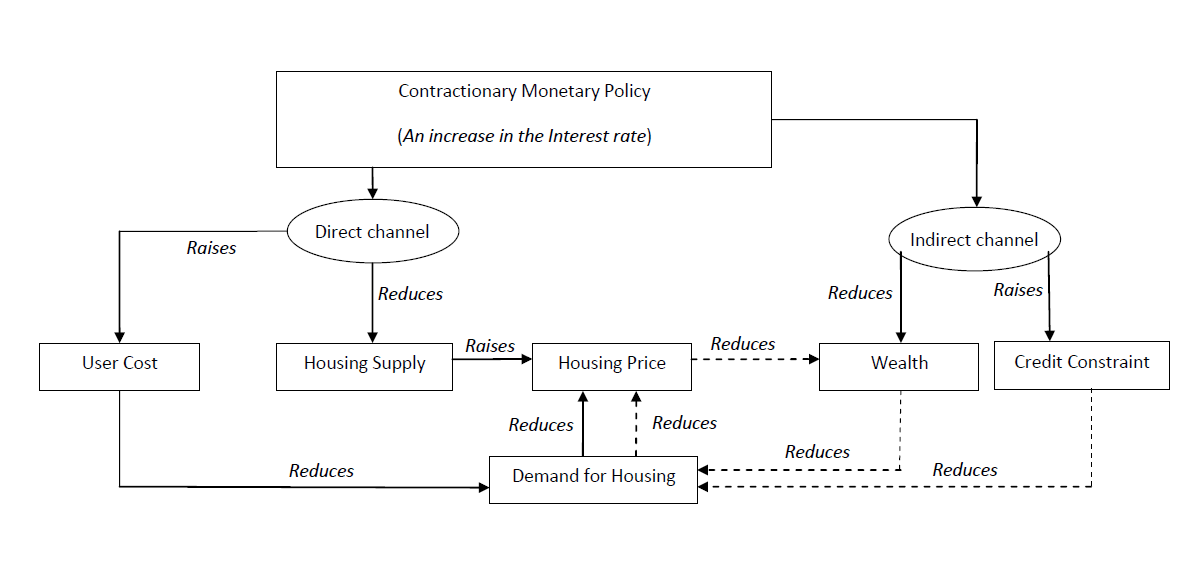
\includegraphics[width=0.9\textwidth]{HousingTransmission}
\\
\cite[Source: See][]{Wadud2009}
\end{figure}

Following his older paper on monetary transmission channels, Mishkin concentrates merely on housing market in his more recent paper~\footcite[See.][]{Mishkin1996} and explains these channels as follows:
\subsubsection{Direct Channels}
Direct Interest Rate Effects through the User Cost of Capital

The user cost of housing capital can be described as ~\footcite[See.][]{Mishkin2007}
 \[ uc = hp((1-t)i - \pi_e) - (/pi_h - /pi_e) + \delta \]
 whre $uc$ is user cost of capital, $hp$ is the relative purchase price of new housing capital, $i$ is the mortgage rate and $/pi_h$ and $/pi_e$ are the appreciation of housing prices and real inflation. $\delta$ is depreciation rate for housing. The formula also deductible mortgage interest by adjusting the nominal mortgage rate by the marginal tax rate $t$. after tax real interest rate. One can see that when the interest rate raises the user cost of capital raises  and consequently the demand for housing decreases. The fall in demand result in a fall in supply and consequently aggregate demand. Looking more precisely in $(/pi_h - /pi_e)$ part of user cost equation one can see the effect of interest rate. When interest rate raises the expected appreciation of housing price falls and therefore the current user cost of capital increases which in turn result in decline in demand. 

Interest Rate Effect on Supply \footcite[See.][]{Mishkin2007}
Higher short-term rates, which increase cost of supply and decreases housing activity.

\subsubsection{Indirect Channels}
Wealth Effects \footcite[See.][]{Mishkin2007}
There evidences proving an increase in wealth should have positive effect on consumption\footcite[See.][]{Mishkin2007}. As we know from previous section an expansionary monetary policy can increase the demand for housing which normally leads to in increase in house price. Therefore, this results to an increase in total wealth and consequently aggregate demand.
Balance Sheet, Credit-Channel Effects on Consumer Spending \footcite[See.][]{Mishkin2007}
An increase in house price improves the house hold balance sheet and reduces the risk for the credit giver as explained in previous sections.



\subsection{Objectives}
In this paper we try to explain the relationship between housing price and monetary and fiscal policies implemented in Germany .
The major objectives of the study are: Firstly, to explain the behavior of the housing market in relationship to monetary policies in Germany using the previously mentioned housing related monetary transmission channels. Secondly, to analyze the data and derive a model using computational macro economics methods (in this case SVAR) method and examine how shocks to different macroeconomics variables affect housing price and housing output.

\subsection{Methodology}
 \subsubsection{Transmission Channels}
Firstly the transmission channels proposed by Mishkin \footcite[See.][]{Mishkin2007} illustrated in Figure \ref{fig:HousingTransmission} are used to explain the macro economics and housing related data in Germany. Secondly, an SVAR model is proposed and identified using the data evidence. 
\subsubsection{SVAR Model Identification}
The structural VAR modeling is one of the standard tools in computational macro economics. In this work we Modify the model used by Wadud \cite[Source: See][]{Wadud2009} and suggest the following model to be identified.
\[ A_0 Y_t = A_1(L) Y_t + B \epsilon_t \]

 If $n$  is the number of variables in the model then $A_0$ and $B$ are $n * n$ matrices and $A_1(L)$ is the matrices polynomial in the lag operator in which $A$ matrices have the same size as $A_0$ matrix.

The assumed $Y$ is :
\[ 
 \begin{bmatrix}
        ry \\ 
        \pi \\
        rg \\
        r \\
        mc \\
        h \\
        rhp \\
  \end{bmatrix}
\]
Where variables are in turn r
real gdp from bundes bank
 change in consumer price index Calendar and seasonally adjusted  rate from bundes bank to remove short term trends (2015 = 100)
(source: bundes bank https://www.bundesbank.de/dynamic/action/en/statistics/time-series-databases/time-series-databases/759784/759784?listId=www_s311_lr_vpi)

r is the money market interest rate (EONIA) ate at which banks provide loans to each other with a duration of 1 day, In my opinion this is a good indicator of the monetary policy since it combines central banks ECB's deposit facility rate and ECB interest rates for main refinancing operations. This affect is more clear when we look in the recent data after 2018 where central banks interest rate for refinancing is zero but the deposit facility goes negative and this stimulates banks to lend more money. 

rg is
General government deficit(-) or surplus(+) as defined in the Maastricht Treaty from  Bundes Bank is used, In my opinion it is a good indicator of the Government fiscal policy since it includes both expenditure and earinging of the gorvernment.

ry is
Germany / National accounts / Overall economy / Gross domestic product (price adjusted) 1, 2, 3

rhp is 
Real house prices, 2015=100, adjusted! https://data.oecd.org/price/housing-prices.htm

mc 
change in percent Construction price index / Germany / Unadjusted figure / Total  bundes bank

h
west germany is used as trend is the same in east! this is the only free source of data I could find for this period.
 https://www.statista.com/statistics/999254/number-completed-new-dwellings-west-germany/ in thousenad


 real government expenditure from bundes bank
 material cost index from Bundes Bank
 housing price index and from Bundes Bank
 real housing price index from Bundes Bank


